\documentclass[]{article}
\usepackage[hyphens]{url}
\usepackage[pdfusetitle,colorlinks,plainpages]{hyperref}
\usepackage[dutch]{babel}
\usepackage{lipsum} % for dummy text only
\usepackage{csquotes}
\usepackage[backend=bibtex]{biblatex}
%\usepackage[acronym]{glossaries}
\usepackage{eurosym}
\usepackage{subfigure}
\usepackage{multirow}
\usepackage{tikz}
\usepackage{listings}
\usepackage{caption}
\usepackage{pdfpages}

\usepackage{todonotes}
\usepackage{placeins}

\usepackage{tikz}
\usepackage{pgfplots}
\usepackage{verbatim}

%opening
\title{IMP: MongoDB}
\author{Thomas Uyttendaele}

\begin{document}

\maketitle
\section{Algemene inleiding}
In deze sectie zal voor de verschillende systemen de automatisering van installatie en configuratie met behulp van IMP uitgelegd worden. Er zal steeds de afhankelijkheden gegeven worden, een domeinmodel, uitleg bij het domeinmodel en voorbeeld configuratie gegeven worden. 

De automatisatie van installatie is ontwikkeld en getest met Fedora 18 en 20, op andere distributies en versies is er niet getest. 
Elk systeem maakt gebruik van \textit{ip::services::Server}, een instantie hiervan is een (virtuele) machine met een IP adres en besturingssysteem. 

Bij elke instantie is het verplicht om de firewall uit te zetten en SELinux op permissive te zetten. Dit kan met behulp van de volgende commando's: 
\begin{lstlisting}[frame=single, breaklines=true]
systemctl stop firewalld.service  
systemctl disable firewalld.service  
setenforce 0
sed -i "s/SELINUX=enforcing/SELINUX=permissive/g" /etc/sysconfig/selinux
sed -i "s/SELINUX=enforcing/SELINUX=permissive/g" /etc/selinux/config|
\end{lstlisting}

\section{MongoDB}
\textit{Link: \url{https://github.com/thuys/mongodb}}

Benodigde IMP modules: std, net, ip, redhat, hosts en yum. 

De installatie en configuratie is gebeurd aan de hand van de uitleg en yum-repository van MongoDB\footnote{\url {http://docs.mongodb.org/manual/tutorial/install-mongodb- on-red-hat-centos-or-fedora-linux/}, \url{http://docs.mongodb.org/manual/tutorial/deploy-replica-set-for-testing/} en  \url{http://docs.mongodb.org/manual/tutorial/deploy-shard-cluster/}}. 

\subsection{Domein model en uitleg}
Het domeinmodel is te zien in figuur \ref{fig:imp-mongodb-domeinmodel}.

	\paragraph{MongoDB} is een server in het IMP model en is verantwoordelijk voor het installeren van de basis van MongoDB. Hierna zijn basis commando's voor connectie te maken met een MongoDB instantie beschikbaar. 
	\paragraph{MonogDBServer} is een server in het IMP model en is verantwoordelijk voor het installeren van de MongoDB server. 
	\paragraph{MongoDBNode} is de implementatie van een data instantie, maximaal 1 per server. Indien gelinkt met een replica set zal deze als een deel van een replica set worden geïnitialiseerd, anders als een zelfstandige instantie. 
	\paragraph{MongoDBReplicaSet} is de voorstelling van een replica set, dit wordt niet aan een specifieke server toegewezen. 
	\paragraph{MongoDBReplicaSetController} is verantwoordelijk om de replica set te initialiseren. Belangrijk is dat indien er een uitbreiding is van de set, de node verbonden met de controller een reeds geïnitialiseerde node is.  
	\paragraph{MongoDBConfigServer} is de implementatie van een configuratie server, 1 of 3 servers zijn nodig per cluster. 
	\paragraph{MongoDBAccessServer} is de implementatie van mongos, minstens 1 is nodig maar meer kunnen gebruikt worden.
	\paragraph{MongoDBShardCluster} is de voorstelling van een cluster van shards, er kunnen zowel alleenstaand instanties als replica sets aan toegevoegd worden. 
	\paragraph{MongoDBShardController} is verantwoordelijk om de cluster te initialiseren met de verschillende shards, databases, collecties en keys. 
	\paragraph{MongoDBDatabase} is de voorstelling van een database.
	\paragraph{MongoDBCollection} is de voorstelling van een collectie, indien verbonden met een cluster via een database zal deze gedeeld worden over de verschillende shards. 
	\paragraph{MongoDBKey} is de wijze waarmee een collectie verdeeld wordt over de verschillende shards. 

\begin{figure}[ht!]
\centering
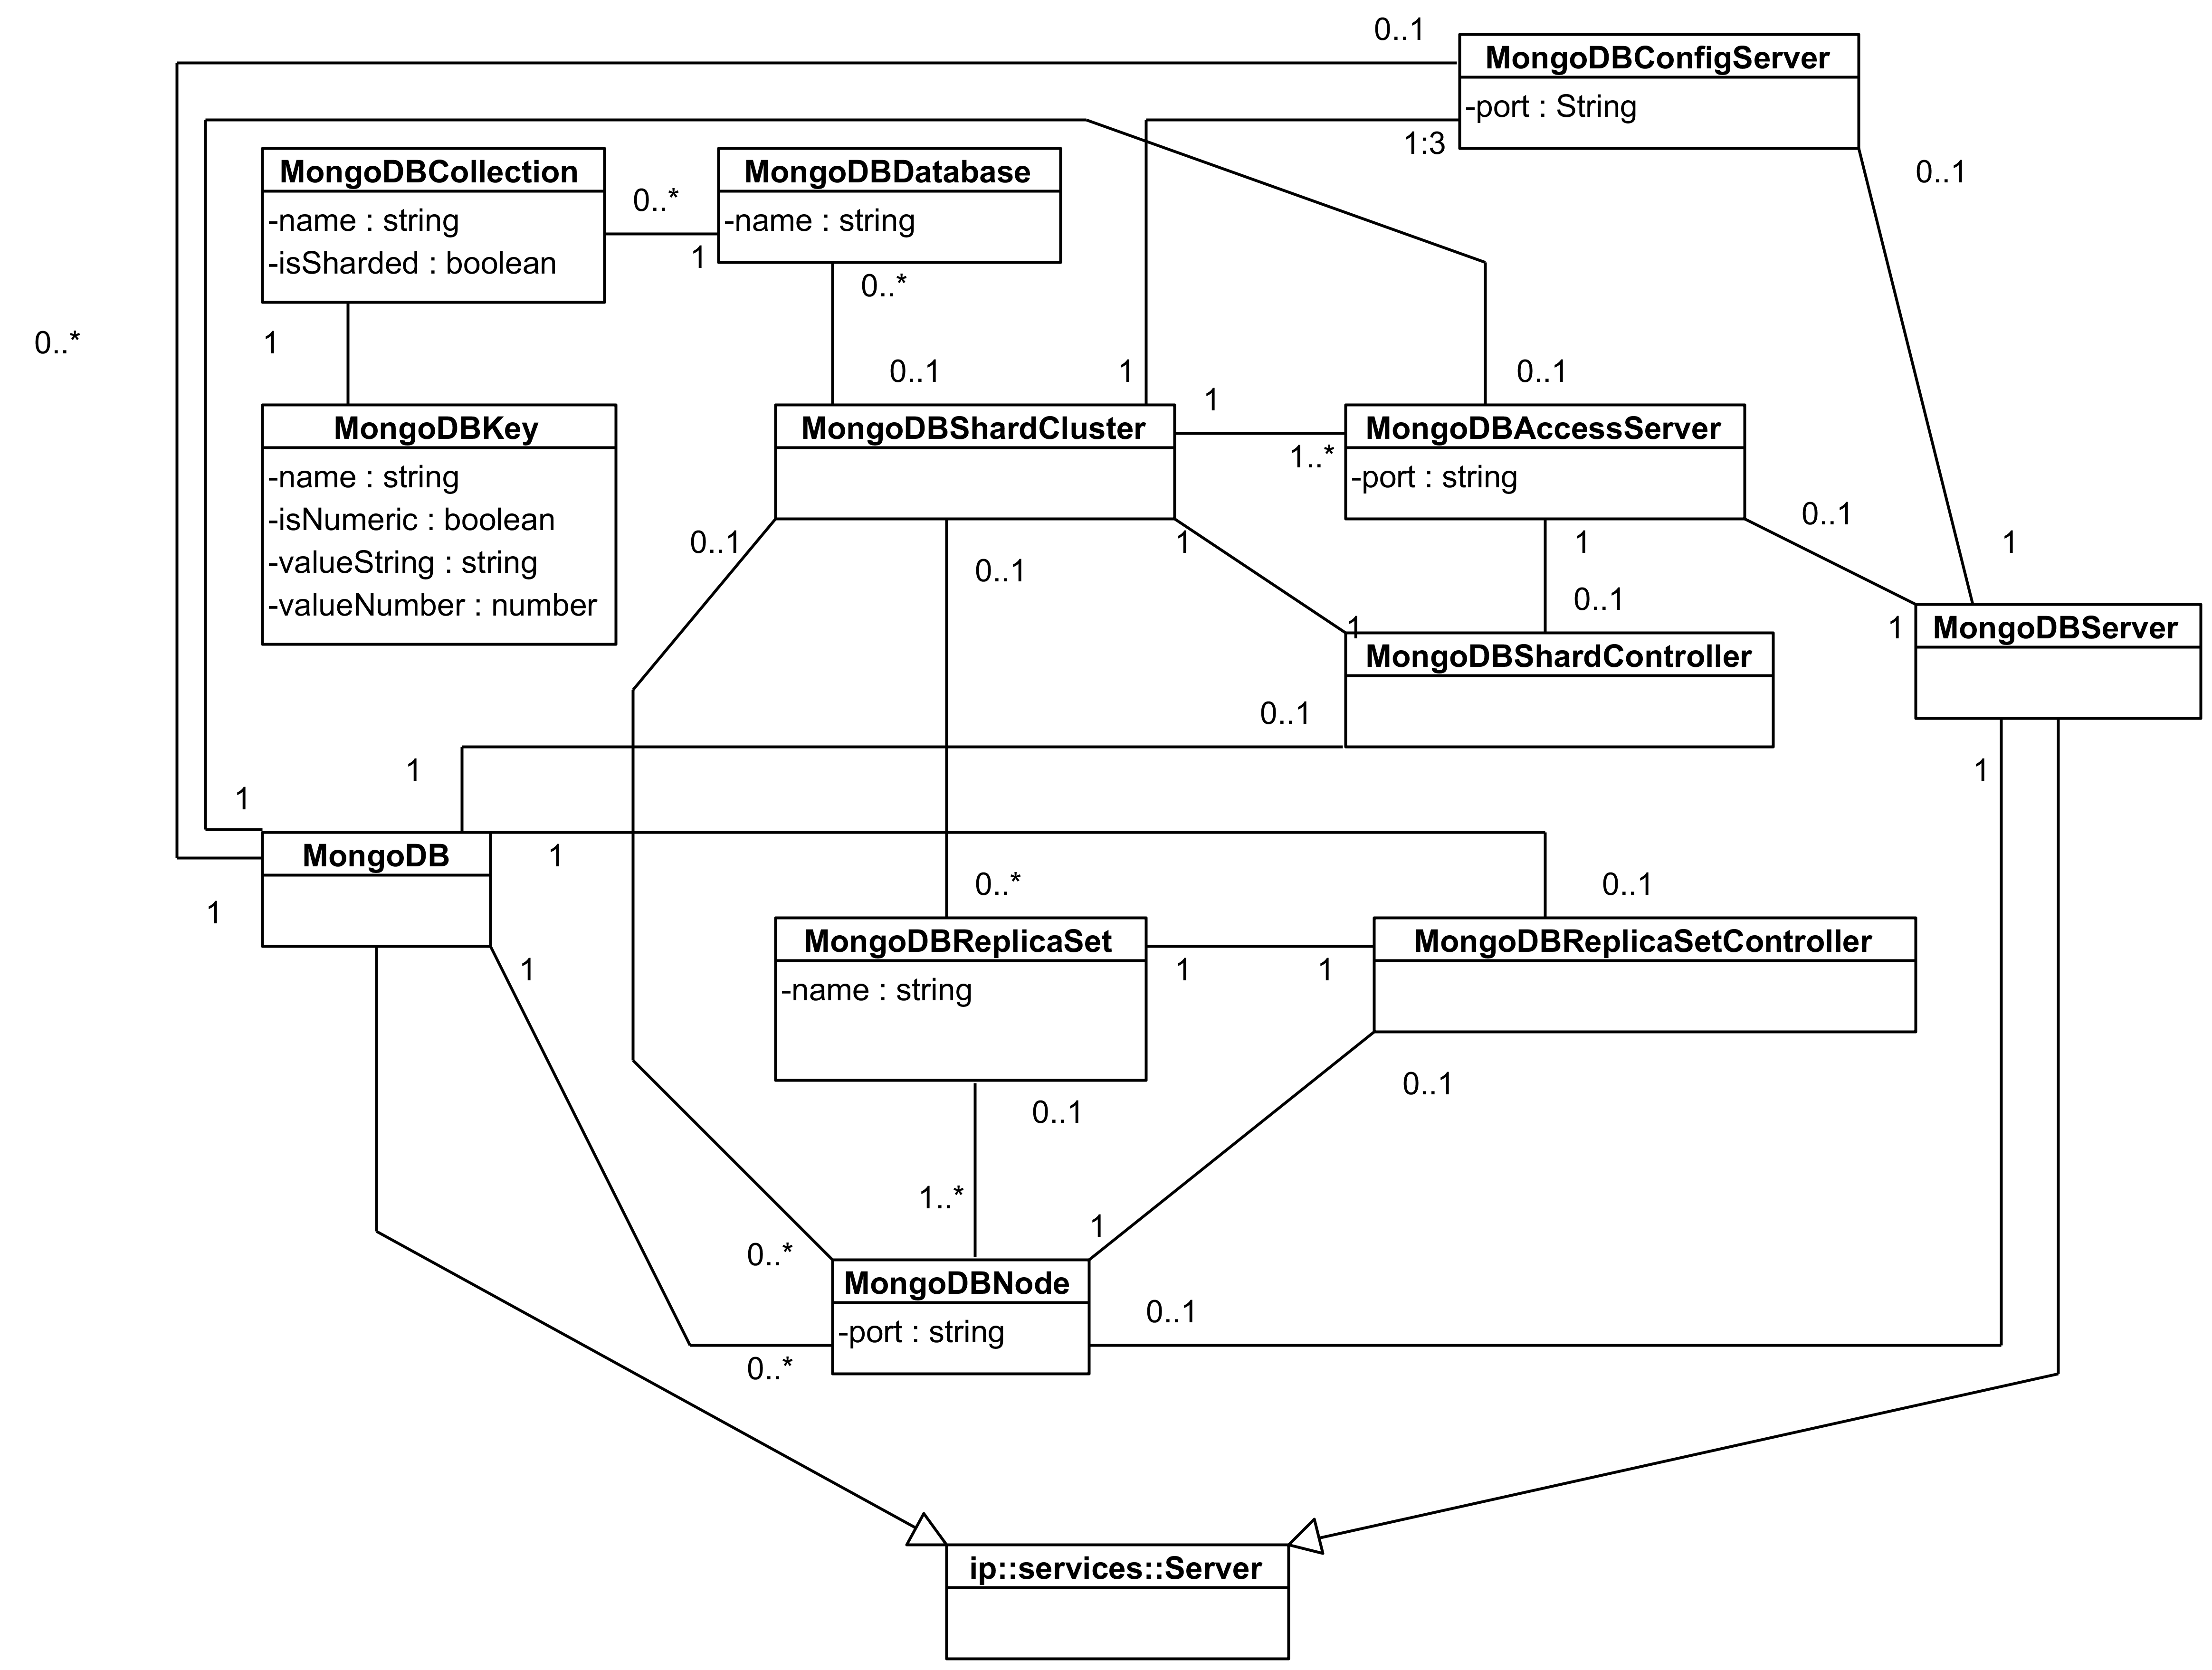
\includegraphics[width=\linewidth]{img/MongoDB-Domeinmodel.png}
\caption{MongoDB: Domeinmodel MongoDB in IMP}
\label{fig:imp-mongodb-domeinmodel}
\end{figure}

\subsection{Voorbeeld configuratie}
De configuratie voor de testomgeving gaat als onderstaand. Bij de uitrol van IMP gaat dit verschillende keren uitgevoerd moeten worden omdat eerst de MongoDBNodes moeten draaien, vervolgens kunnen de replicasets aangemaakt worden, daarna kunnen de replicasets pas toegevoegd worden in de cluster. 

In IMP was het nog niet mogelijk om een te zeggen dat x uitgevoerd moet zijn op een andere instantie, vooraleer y kan uitgevoerd worden, ondertussen is dit mogelijk door de thesis van Harm De Weirdt\cite{thesisHarm} waar de nieuwe installatie beschikbaar is op \url{https://github.com/Foezjie/mongodb} maar hierbij dient ook gebruik gemaakt te worden van zijn IMP installatie.  \\
Met het ontbreken hieraan kan het zijn dat er 3 keer een volledige IMP deploy uitgevoerd moet worden. 

\lstinputlisting[language=Python, breaklines=true, frame=single]{code/imp-mongodb.conf}
\end{document}
